Residual graphs $G_f = \mathcal{E} \ominus f$ 

\begin{figure}[ht]
	\caption[Maximum Flow]{
	Loooooooooooooooonnnng Caption.
	}
	\label{fig:maxflow}
	\centering
	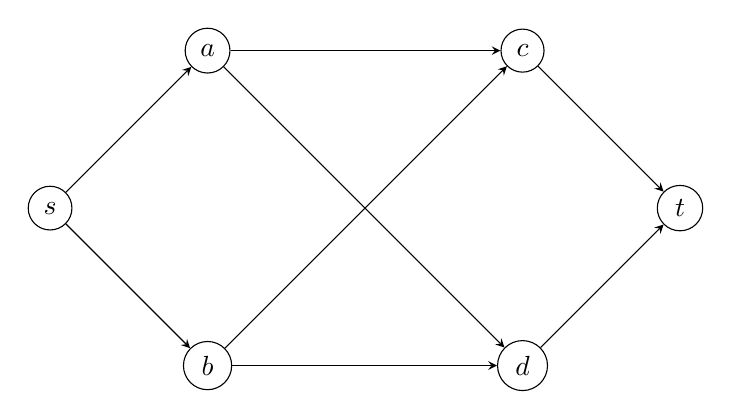
\begin{tikzpicture}[scale=2]
		\draw (0,0) node[draw, circle] (S) {$s$};
		\draw (1,1) node[draw, circle] (A) {$a$};
		\draw (1,-1) node[draw, circle] (B) {$b$};
		\draw (3,1) node[draw, circle] (C) {$c$};
		\draw (3,-1) node[draw, circle] (D) {$d$};
		\draw (4,0) node[draw, circle] (T) {$t$};
		\draw[->, >=stealth] (S) -- (A);
		\draw[->, >=stealth] (S) -- (B);
		\draw[->, >=stealth] (A) -- (C);
		\draw[->, >=stealth] (B) -- (C);
		\draw[->, >=stealth] (B) -- (D);
		\draw[->, >=stealth] (A) -- (D);
		\draw[->, >=stealth] (C) -- (T);
		\draw[->, >=stealth] (D) -- (T);
	\end{tikzpicture}
\end{figure}
	
This can be used to formulate a ``reversed'' Ford-Fulkerson algorithm.
Rather than start with an empty flow, start with $f = \mathcal{E}$, a full-capacity ``flow''.
It is unlikely that $f$ will initially be a valid flow.
